\documentclass[tikz]{standalone}

\usepackage{stanli}

\begin{document}
	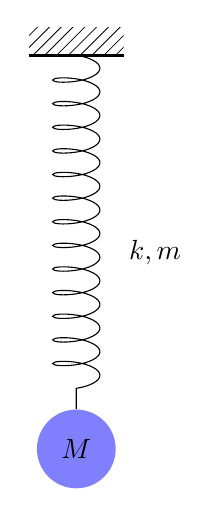
\begin{tikzpicture}
		[defsty/.style={circle ,fill=blue!50, minimum size=1cm},
		arcsty/.style={
			decoration={coil,aspect=0.3,segment length=3mm,amplitude=3mm},
			decorate, draw}]
			
		\point{a}{0}{0};
		\support{3}{a}[180];
		
		\coordinate (A) at (0,0);
		\node[defsty] (B) at (0, -5) {$M$};
		\node[fill=white, line width=0] (C) at (1,-2.5) {$k,m$};
		
		\draw[arcsty] (A) -- (B);
	\end{tikzpicture}
\end{document}